\documentclass[a4paper,12pt]{article} % добавить leqno в [] для нумерации слева
\usepackage[a4paper,top=1.3cm,bottom=2cm,left=1.5cm,right=1.5cm,marginparwidth=0.75cm]{geometry}
%%% Работа с русским языком
\usepackage{cmap}					% поиск в PDF
\usepackage{mathtext} 				% русские буквы в фомулах
\usepackage[T2A]{fontenc}			% кодировка
\usepackage[utf8]{inputenc}			% кодировка исходного текста
\usepackage[english,russian]{babel}	% локализация и переносы


\usepackage{graphicx}

\usepackage{wrapfig}
\usepackage{tabularx}

\usepackage{hyperref}
\usepackage[rgb]{xcolor}
\hypersetup{
colorlinks=true,urlcolor=blue
}
\usepackage{multirow}
\usepackage{hhline}


%%% Дополнительная работа с математикой
\usepackage{amsmath,amsfonts,amssymb,amsthm,mathtools} % AMS
\usepackage{icomma} % "Умная" запятая: $0,2$ --- число, $0, 2$ --- перечисление

%% Номера формул
\mathtoolsset{showonlyrefs=true} % Показывать номера только у тех формул, на которые есть \eqref{} в тексте.

%% Шрифты
\usepackage{euscript}	 % Шрифт Евклид
\usepackage{mathrsfs} % Красивый матшрифт

%% Свои команды
\DeclareMathOperator{\sgn}{\mathop{sgn}}

%% Перенос знаков в формулах (по Львовскому)
\newcommand*{\hm}[1]{#1\nobreak\discretionary{}
{\hbox{$\mathsurround=0pt #1$}}{}}

\begin{document}
	
	\begin{titlepage}
	\begin{center}
		{\large МОСКОВСКИЙ ФИЗИКО-ТЕХНИЧЕСКИЙ ИНСТИТУТ (НАЦИОНАЛЬНЫЙ ИССЛЕДОВАТЕЛЬСКИЙ УНИВЕРСИТЕТ)}
	\end{center}
	\begin{center}
		{\large Физтех-школа электроники, фотоники и молекулярной физики}
	\end{center}
	
	
	\vspace{4.5cm}
	{\huge
		\begin{center}
			{Лабораторная работа 4.4.4}\\
			Интерферометр Фабри-Перо
		\end{center}
	}
	\vspace{2cm}
	\begin{flushright}
		{\LARGE Салтыкова Дарья \\
			\vspace{0.5cm}
			Б04-105}
	\end{flushright}
	\vspace{8cm}
	\begin{center}
		Долгопрудный 2023
	\end{center}
\end{titlepage}

\section{Введение}

\noindent \textbf{Цель работы:} измерение длины волны жёлтых линий ртути, жёлтого дублета натрия, определение спектральных характеристик интерферометра Фабри—Перо.

\medskip
	
\noindent \textbf{В работе используются:} интерферометр Фабри—Перо, линзы, светофильтры, ртутная и натриевая лампы, катетометр КН-6.
		

\section{Экспериментальная установка}

Схема экспериментальной установки представлена на рис. 1. Свет от ртутной лампы $ S $, пройдя через линзу $ Л_0 $ и светофильтр $ C $, попадает на интерферометр Фабри-Перо (ИФП). Линза $ Л_0 $ служит для
	формирования пучка лучей (слегка сходящегося или слегка расходящегося). Интерференционные кольца наблюдаются в локальной плоскости линзы $ Л $. Картина рассматривается через зрительную трубу $ Т $, сфокусированную на эту плоскость. Диаметры колец измеряются с помощью микроскопа катетометра.
	
		\begin{figure}[h!]
		\centering
		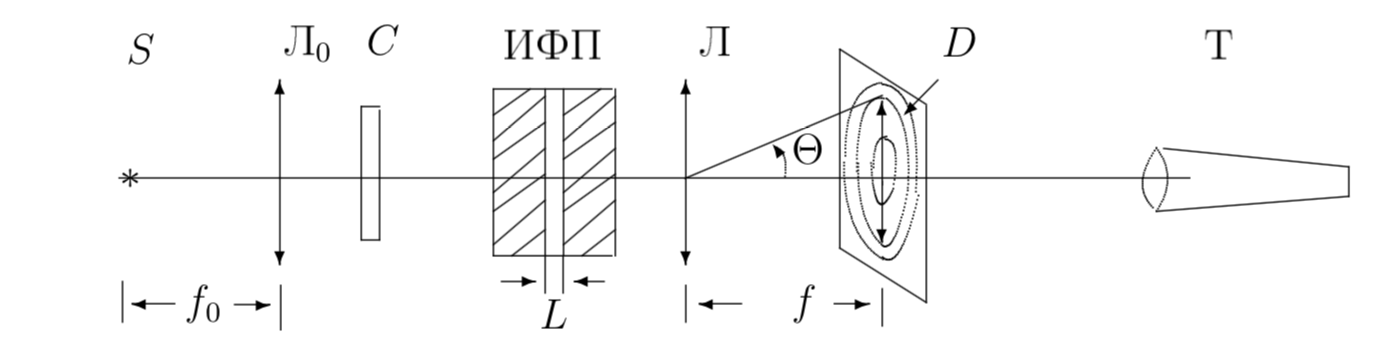
\includegraphics[width=\linewidth]{lab.png}
		\caption{Экспериментальная установка}
		\label{lab}
	\end{figure}

	
\noindent Зрительная труба $ Т $ и отсчетный микроскоп  --- элементы катетометра --- прибора, предназначенного для измерения расстояний в вертикальной плоскости вдоль вертикальной оси. 
	При достаточной яркости ртутной лампы можно увидеть, что зелёная линия
	ртути состоит из нескольких компонентов. Расщепление этой спектральной линии связано с дополнительной энергией, возникающей как в результате взаимодействия магнитных моментов ядра и электрона --- \textit{сверхтонкая структура} (магнитное поле ядра действует на спиновый магнитный момент электрона), так и с \textit{изотопическим сдвигом} (в парах ртути присутствуют в заметных количествах изотопы с атомными массами от 198 до 204 а.е.м.). Каждое зелёное кольцо содержит более десятка близко расположенных компонентов, но разрешение нашего прибора не позволяет все их рассмотреть.
	
\medskip	
	
\noindent Спектр натриевой лампы исследуется по аналогичной схеме, но светофильтр в этом случае не нужен, а интерферометр, линзы и зрительная труба катетометра
	имеют другие параметры.

\section{Ход работы}

\subsection{Ртутная лампа}
		
\noindent Проведем измерения диаметров зеленых и желтых интерференционных колец с помощью катетометра, оценивая его погрешность измерения как $ \sigma_a = 0,3 $ мм. Параметр установки --- фокусное расстояние линзы $ f = 110 $ мм.
		
\medskip		
		
\noindent Будем последовательно измерять расстояния от верхнего края 6-ого "<набора"> колец до нуля (центра), затем аналогично будем измерять расстояния от нижнего края до нуля. Результаты занесем в таблицы. 
		
			\begin{table}[]
\begin{tabular}{|lllll|}
\hline
\multicolumn{5}{|c|}{зеленые}                                                                                                                                                            \\ \hline
\multicolumn{1}{|l|}{i} & \multicolumn{1}{l|}{$a_{\text{в}}, \text{ мм}$} & \multicolumn{1}{l|}{$a_{\text{н}}, \text{ мм}$} & \multicolumn{1}{l|}{$D, \text{ мм}$} & $D^2, \text{ мм}^2$ \\ \hline
\multicolumn{1}{|l|}{6} & \multicolumn{1}{l|}{189,97}                     & \multicolumn{1}{l|}{159,02}                     & \multicolumn{1}{l|}{30,95}           & 957,9025            \\ \hline
\multicolumn{1}{|l|}{5} & \multicolumn{1}{l|}{188,76}                     & \multicolumn{1}{l|}{160,62}                     & \multicolumn{1}{l|}{28,14}           & 791,8596            \\ \hline
\multicolumn{1}{|l|}{4} & \multicolumn{1}{l|}{187,56}                     & \multicolumn{1}{l|}{162,28}                     & \multicolumn{1}{l|}{25,28}           & 639,0784            \\ \hline
\multicolumn{1}{|l|}{3} & \multicolumn{1}{l|}{186,57}                     & \multicolumn{1}{l|}{164,53}                     & \multicolumn{1}{l|}{22,04}           & 485,7616            \\ \hline
\multicolumn{1}{|l|}{2} & \multicolumn{1}{l|}{184,12}                     & \multicolumn{1}{l|}{166,7}                      & \multicolumn{1}{l|}{17,42}           & 303,4564            \\ \hline
\multicolumn{1}{|l|}{1} & \multicolumn{1}{l|}{181,2}                      & \multicolumn{1}{l|}{169,65}                     & \multicolumn{1}{l|}{11,55}           & 133,4025            \\ \hline
\end{tabular}
\end{table}

\begin{table}[]
\begin{tabular}{|lllllll|}
\hline
\multicolumn{7}{|c|}{желтые}                                                                                                                                                                                                                                                                                                 \\ \hline
\multicolumn{1}{|l|}{i} & \multicolumn{1}{l|}{$a_{1 \text{в}}, \text{ мм}$} & \multicolumn{1}{l|}{$a_{1 \text{н}}, \text{ мм}$} & \multicolumn{1}{l|}{$a_{2 \text{в}}, \text{ мм}$} & \multicolumn{1}{l|}{$a_{2 \text{в}}, \text{ мм}$} & \multicolumn{1}{l|}{$\overline{D}, \text{ мм}$} & $\frac{1}{\Delta D}, \text{ мм}$ \\ \hline
\multicolumn{1}{|l|}{1} & \multicolumn{1}{l|}{182,53}                       & \multicolumn{1}{l|}{171,32}                       & \multicolumn{1}{l|}{179,78}                       & \multicolumn{1}{l|}{173,85}                       & \multicolumn{1}{l|}{8,57}                       & 0,1893939                        \\ \hline
\multicolumn{1}{|l|}{2} & \multicolumn{1}{l|}{186,65}                       & \multicolumn{1}{l|}{166,98}                       & \multicolumn{1}{l|}{185,53}                       & \multicolumn{1}{l|}{168,22}                       & \multicolumn{1}{l|}{18,49}                      & 0,4237288                        \\ \hline
\multicolumn{1}{|l|}{3} & \multicolumn{1}{l|}{189,61}                       & \multicolumn{1}{l|}{164,27}                       & \multicolumn{1}{l|}{188,64}                       & \multicolumn{1}{l|}{164,99}                       & \multicolumn{1}{l|}{24,495}                     & 0,591716                         \\ \hline
\multicolumn{1}{|l|}{4} & \multicolumn{1}{l|}{191,84}                       & \multicolumn{1}{l|}{161,74}                       & \multicolumn{1}{l|}{191,13}                       & \multicolumn{1}{l|}{162,47}                       & \multicolumn{1}{l|}{29,38}                      & 0,6944444                        \\ \hline
\multicolumn{1}{|l|}{5} & \multicolumn{1}{l|}{194,1}                        & \multicolumn{1}{l|}{159,71}                       & \multicolumn{1}{l|}{193,28}                       & \multicolumn{1}{l|}{160,19}                       & \multicolumn{1}{l|}{33,74}                      & 0,7692308                        \\ \hline
\multicolumn{1}{|l|}{1} & \multicolumn{1}{l|}{181,2}                        & \multicolumn{1}{l|}{169,65}                       & \multicolumn{1}{l|}{11,55}                        & \multicolumn{1}{l|}{133,4025}                     & \multicolumn{1}{l|}{}                           &                                  \\ \hline
\end{tabular}
\end{table}


\noindent Построим графики для зеленых и желтых колец:

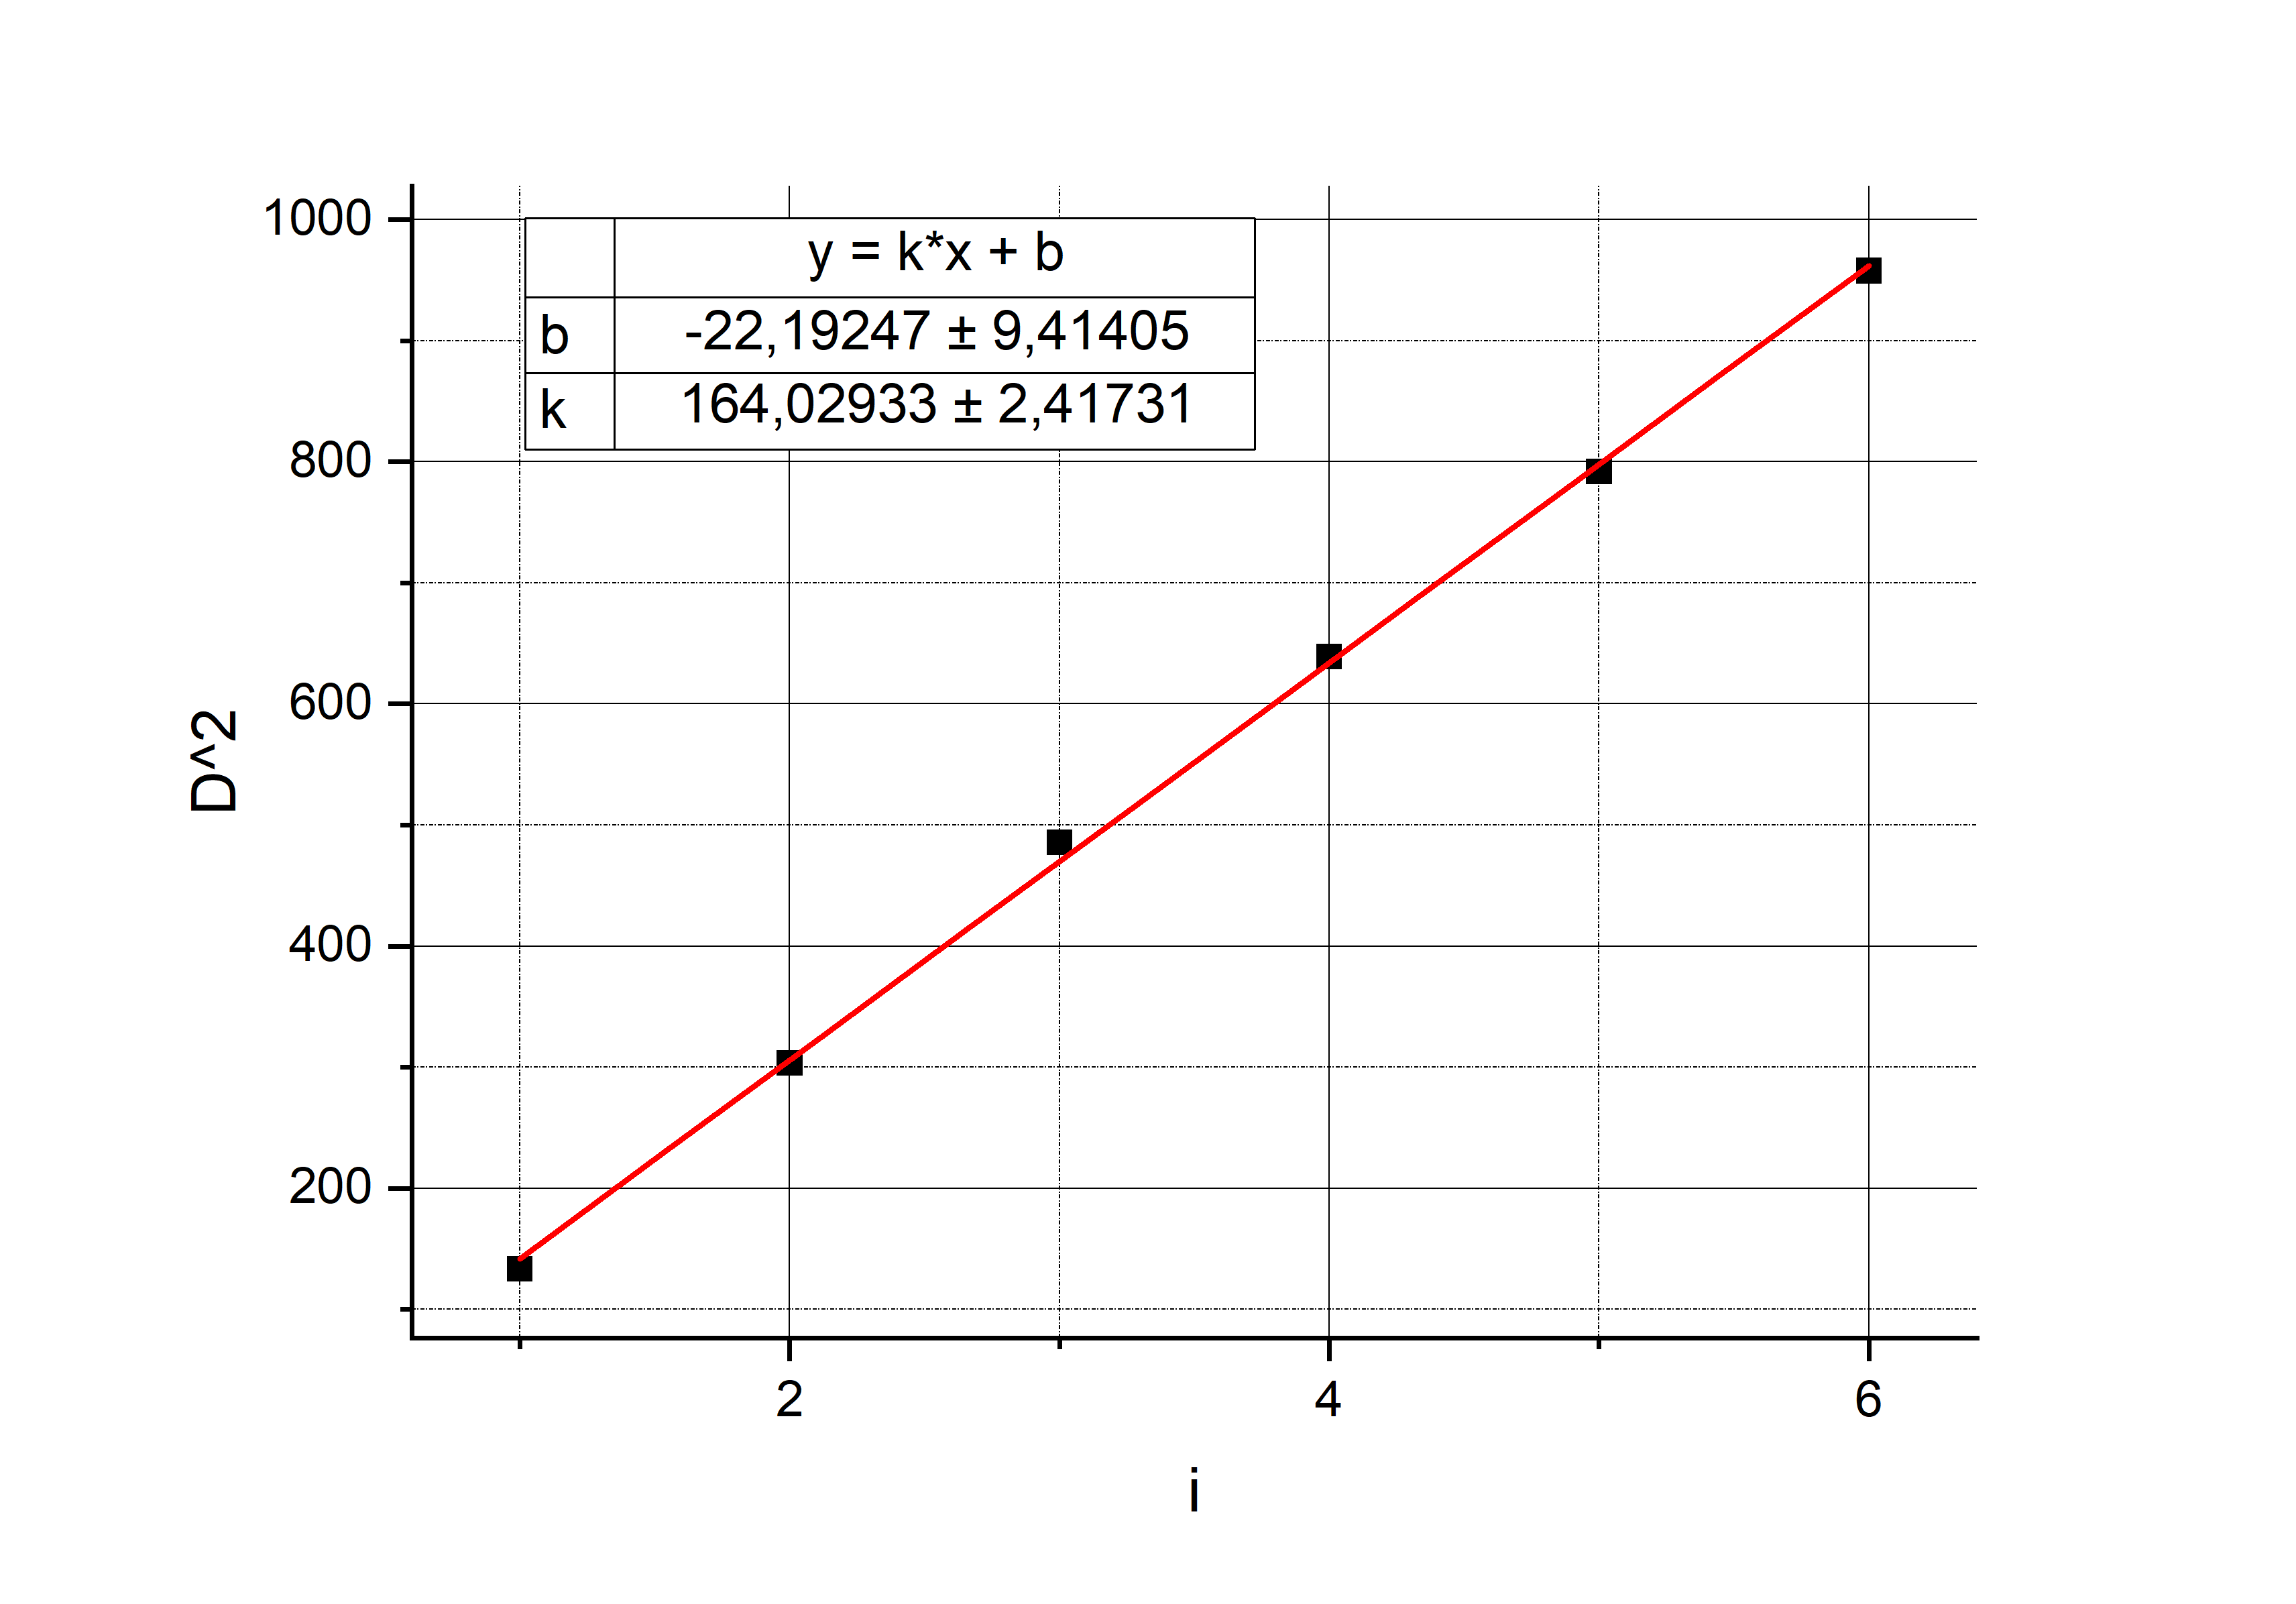
\includegraphics[width=0.9\linewidth]{gr1.png}

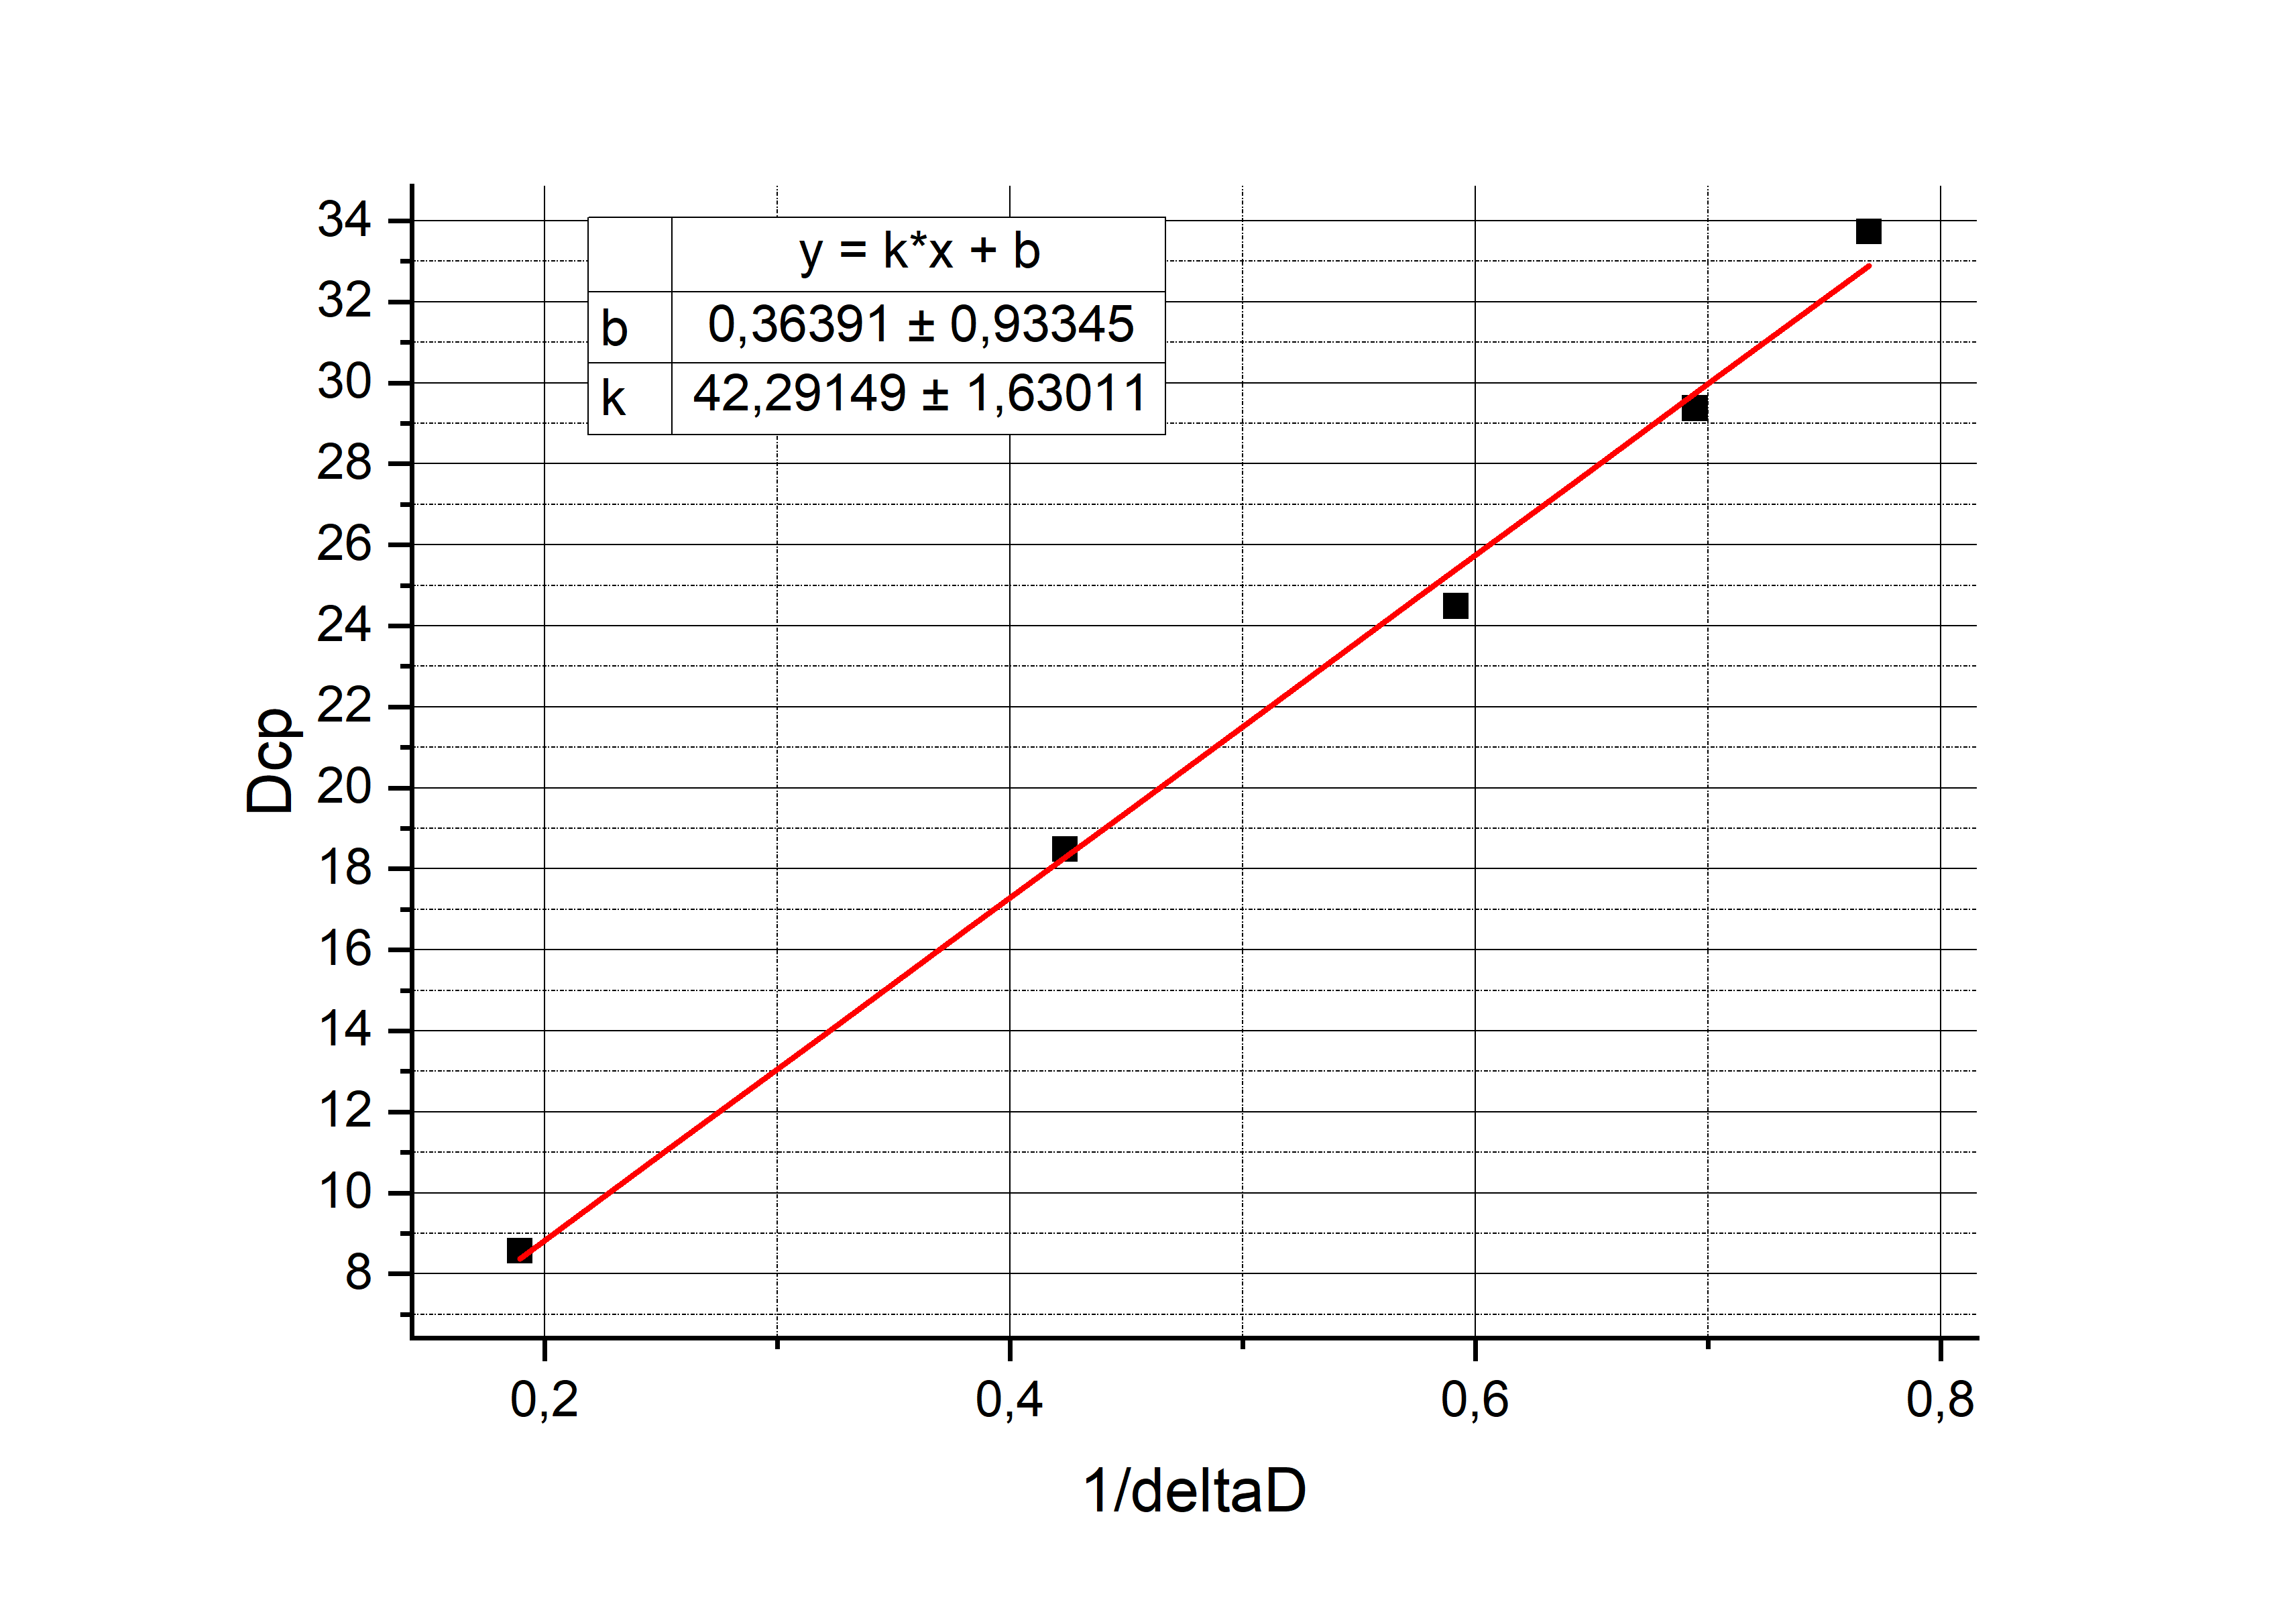
\includegraphics[width=0.9\linewidth]{gr2.png}

\noindent Используя значение средней длины волны зелёной линии ртути $\lambda_{\text{з}} = 5461 \text{\AA}$, определим базу интерферометра L.

 $$ k = \lambda / L = 164\pm 2 $$
\begin{equation*}\label{key}
	L=\frac{4 f^2 \lambda}{k} = (0.16 \pm 0.01)\; \text{мм},
\end{equation*}

\noindent Определим разность длин волн для пары жёлтых линий ртути.

\begin{equation*}\label{key}
	\Delta \lambda = \frac{\lambda \overline{D} \Delta D}{4 f^2} = \frac{\lambda k}{4f^2} = (4.8 \pm 0.2) \; \SI{}\text{\AA}
\end{equation*}

\noindent Оценим максимальный порядок интерференции:

\[
m_\text{жёл} = \frac{2L \cos \theta}{\lambda} \approx \frac{2L}{\lambda} = 590
\]

\noindent Разрешающая способность:

\begin{equation*}\label{key}
	 \delta r = (0.8 \pm 0.01) \;  \text{мм} 
\end{equation*}
\[ R = \frac{4f^2}{D \delta r} = 5240 \pm 100 \]

 

\end{document}